\section{Datenanalyse}

\subsection{Dickebestimmung der Mylar-Folien}
\label{sec:dicke}

Um die Dicken der Mylar-Folien zu bestimmen, werden zunächst die Restenergien der Teilchen nach Passieren der Folien bestimmt.
Dazu wird der $\Delta E$ - Detektor aus dem Strahlengang gedreht und das Energiespektrum der transmittierten Teilchen aufgenommen.
Als Referenz wird hier die Kalibrationsmessung ohne Folie verwendet.
In \cref{fig:foliendicke} sind die vier Messungen normiert nebeneinander eingezeichnet.
Alle konkreten Fitparameter der Doppelgausskurven sind in \cref{tab:fitval1} angegeben.
Im Diagramm ist ein einzelner stark abweichender Datenpunkt bei \SI{4000}{\kilo\electronvolt} auffällig, welcher im Folgenden allerdings nicht weiter dis

\begin{figure}[ht]
	\centering
	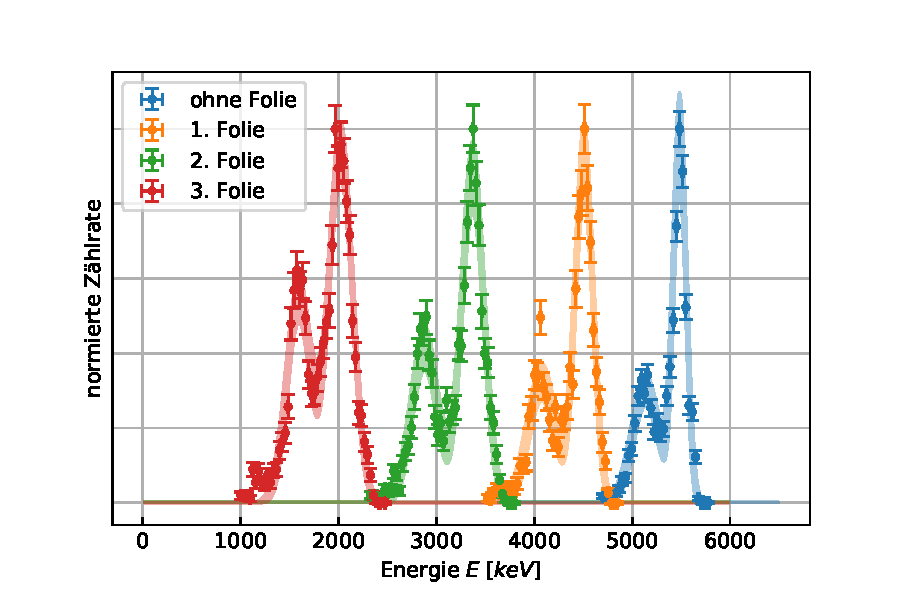
\includegraphics[width=0.7\textwidth]{dat/m3_foliendicke.pdf}
	\caption{Energiespektren nach Passieren der einzelnen Folien.
			Die Zählrate ist normiert, um die Folien besser zu vergleichen.
			Es werden nur die Datenpunkte im Bereich um den Energiepeak ungleich Null angezeigt.
			Über die Daten ist ein Doppelgauss gelegt, welcher die Parameter in \cref{tab:fitval1} annimmt und mit einer Unsicherheit $\pm 3 \sigma$ eingezeichnet ist.}
	\label{fig:foliendicke}
\end{figure}

Für die Analyse sind nur die Positionen der größeren Peaks wichtig.
Diese gehören zur \SI{5485}{\kilo\electronvolt} $\alpha$-Strahlung der Probe.
Der Detektor hat eine begrenzte Messgenauigkeit welche sich durch die Breite der Peaks widerspiegelt.
Um diese zu beachten, wird die Unsicherheit der Position $E_1$ mit der Breite $\sigma_1$ nach Formel (\ref{fig:GUM_combine}) kombiniert.

Nun wird eine numerische Integration durch die Folien durchgeführt.
Dazu wird zunächst der Energieverlust $\dv{E}{x}$ von $\alpha$-Teilchen in Mylar aus der Anleitung interpoliert\footnote{Hierbei wird in python die Funktion \texttt{scipy.interpolate.interp1d} mit dem Parameter \texttt{kind="cubic"} für eine kubische Splineinterpolation genutzt.}.
Für ein eintreffendes Teilchen mit \SI{5485}{\kilo\electronvolt} kann nun schrittweise der Energieverlust $\dd E_i = \dv{E}{x} \left(E_i\right) \cdot \delta x$ berechnet werden.
Es wird so lange integriert, bis die Energie des Teilchens die gemessene Energie unterschritten hat.
Mit $\delta x = \SI{1e-4}{\micro\meter} = \const$ ist die zurückgelegte Strecke $\bar{x} = N \cdot \delta x$, wobei $N$ die Anzahl an benötigten Integrationsschritten ist.
Um die Standardabweichung für die Dicken zu bestimmen, wird die Integration ebenfalls für $E_1^\pm = \bar{E_1} \pm \sigma(E_1)$ durchgeführt.
Nun wird mit den zu $E_1^\pm$ gehörenden Dicken $x^\pm$ die gemittelte Differenz $\sigma(x) = \frac{x^+ - x^-}{2}$ gebildet.
Die ermittelten Energien und Dicken der Folien sind in \cref{tab:dicken} zusammengefasst.

\begin{table}[ht]
	\centering
	\caption{Energien der Teilchen nach Passieren der Folien und die errechneten Dicken dieser.} 
	\label{tab:dicken}
	\begin{tabular}{c|ccc}
		\toprule
		         &          Energie $E_1$          &           Dicke $x$           &  \\ \midrule
		1. Folie & \input{dat/folie_energie_1.txt} & \input{dat/folie_dicke_1.txt} &  \\
		2. Folie & \input{dat/folie_energie_2.txt} & \input{dat/folie_dicke_2.txt} &  \\
		3. Folie & \input{dat/folie_energie_3.txt} & \input{dat/folie_dicke_3.txt} &  \\ \bottomrule
	\end{tabular}
\end{table}

Aus den bestimmten Dicken könnte man schließen, dass die Folien Vielfache von \SI{8}{\micro\meter} dick sind und im Falle der 1. und 2. Folie um ca. \SI{13}{\degree} gedreht sind oder keine gleichmäßige Dicke aufweisen.
Diese Angaben sind allerdings nicht zu überprüfen und sind als Spekulationen zu betrachten.
Um die Unsicherheit zu erhöhen, muss die Detektorgenauigkeit erhöht werden.
Dies kann zum Beispiel über eine Faltung mit der Detektorverteilung einer wohlbekannten Kalibrationsmessung erzielt werden.

\subsection{Bestimmung des Energieverlusts}

Um die Teilchenidentifikation durchzuführen, werden alle aufgenommenen Messungen aufaddiert und in ein Diagramm geschrieben.
Dabei ist die Energie des Teilchens die Summe von gemessener Restenergie im $E$-Detektor und deponierter Energie im $\Delta E$-Detektor.
Die Messdaten, sowie theoretisch errechnete Kurven für Protonen, Deuteronen, Tritonen, Helium-3-Kerne, $\alpha$-Teilchen und Lithium-Kerne sind in \cref{fig:energieverlust} dargestellt.

\begin{figure}[ht]
	\centering
	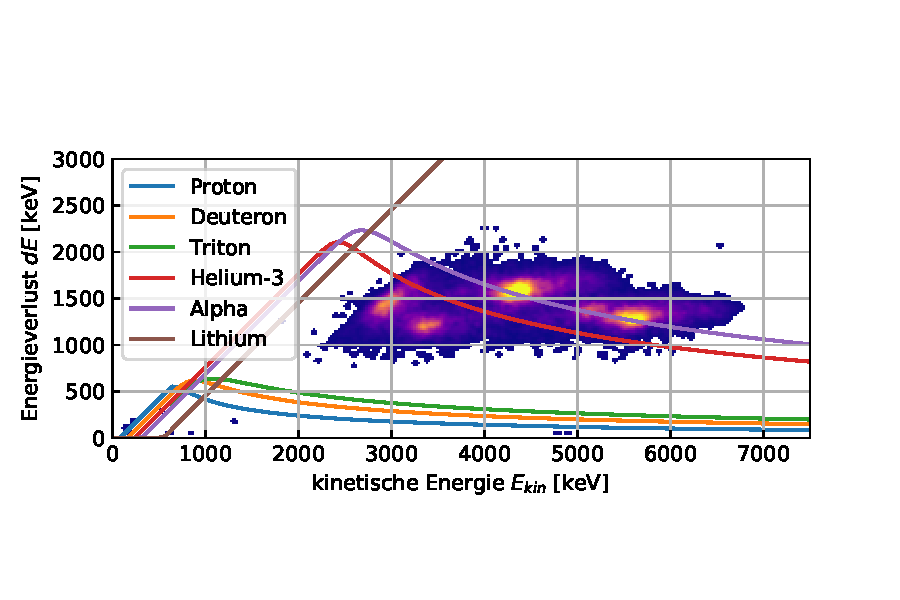
\includegraphics[width=0.7\textwidth]{dat/energieverlust.pdf}
	\caption{Energieverlust $\Delta E$ von Teilchen der Energie $E$. Zusätzlich sind die theoretisch erwarteten Kurven für sechs Teilchensorten eingezeichnet.}
	\label{fig:energieverlust}
\end{figure}

Man kann erkennen, dass die theoretische Kurve für $\alpha$-Teilchen durch die beiden hellsten Punkte sowie durch einen weiteren Häufungspunkt bei $E=\SI{5100}{\kilo\electronvolt}$ verläuft.
Allerdings liegen die beiden Punkte bei $E = \SI{3000}{\kilo\electronvolt}$ und $E=\SI{3400}{\kilo\electronvolt}$ nicht auf der theoretischen Kurve.

Um die theoretischen Kurven zu berechnen, ist die Bethe Bloch Formel nach \cref{eq:bethebloch} für Silikon implementiert worden.
Nun kann wie in \cref{sec:dicke} eine schrittweise Integration durch den Detektor durchgeführt werden.
Die Abbruchbedingung ist diesmal die Dicke des Detektors $d = \SI{8.5257}{\micro\meter}$, welche aus \cref{sec:de_kalibration} bekannt ist. %TODO ref jannik aufgabe 2
